\documentclass[12pt]{article}
\usepackage[spanish, es-tabla]{babel}
%\usepackage[top=2.5cm, bottom=2.5cm,left=2cm, right=2cm]{geometry}
\usepackage[top=1.78cm, bottom=1.78cm,left=1.65cm, right=1.65cm]{geometry}
\usepackage[utf8x]{inputenc}
\usepackage{amsmath}
\usepackage{graphicx}
\setlength{\parindent}{12pt}
\usepackage[colorinlistoftodos]{todonotes}
\usepackage{multicol}
\let\olditemize\itemize
\def\itemize{\olditemize\itemsep=0pt }
\usepackage[hidelinks]{hyperref}

\usepackage[pages=some]{background}
\backgroundsetup{
 scale=1,
 color=black,
 opacity=0.2,
 angle=0,
 contents={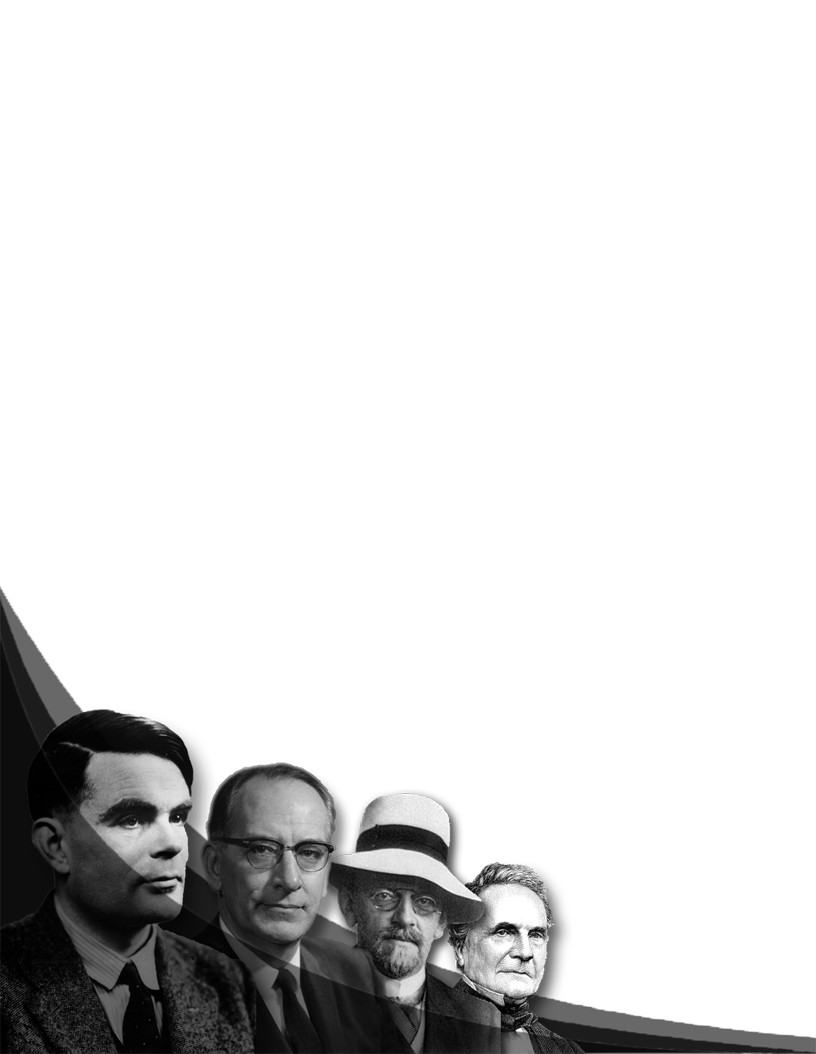
\includegraphics[scale=1]{CORNER.PNG}
 }
}

\begin{document}
\begin{titlepage}
\BgThispage
\newcommand{\HRule}{\rule{\linewidth}{0.5mm}}
\center

\includegraphics[scale=0.4]{Escudo.jpg}\\[0.5 cm]
\textsc{\large Departamento de electrónica}\\[0.5cm]
\textsc{\large Curso de informática II}\\[0.5cm] 
\HRule \\[0.4cm]
{ \huge \bfseries El Bit Bang: \\[0.5 cm]\LARGE De la discordia matemática al orígen de la computación moderna}\\[0.4cm]
\large{por: }\\[0.3cm]
\textsc{Santiago Giraldo Tabares}\\
\HRule \\[1.5cm]
{\LARGE{Medellín, Antioquia, Colombia\\[0.2 cm]Marzo, 2020}}\\
\vfill
\end{titlepage}


\begin{multicols}{2}
%\textsl{“Un lenguaje nuevo, vasto y poderoso se está desarrollando para el uso futuro del análisis, en el cual se pueden introducir sus principios con el fin de que tengan una aplicación práctica más veloz y precisa al servicio de la humanidad.”}\\
%\textbf{\textsl{Ada Lovelace}}
\section*{Introducción}
El siglo XX fue una explosión vertiginosa del pensamiento humano, una época de grandes investigaciones y avances, impulsada por y para la industria. Con esto, germinaron motivaciones que no son más que  adyacentes a una razón, a un génesis tecnológico que aceleró la competitividad académica a la par de las tensiones internacionales: La guerra. En paralelo, la comunidad matemática había alcanzado un punto en el que comenzaban a tocarse temas casi filosóficos, generando incertidumbre sobre el futuro de esta y las demás ciencias que se asientas sobre ella. Analicemos el origen de la computación moderna como el punto de convergencia de las dos siguientes historias.
\section*{1. Las máquinas de análisis:}
La historia de estas es larga. En tanto como queramos considerar todos los ábacos de madera que han existido en las sociedades antiguas.\cite{Flo} Personajes como Blaise Pascal ya habían desarrollado máquinas que mecanizaban el cálculo aritmético. Pero no sería sino hasta 1833 que se registraría la verdadera precursora de la computación moderna: La máquina analítica de Charles Babbage. Pero, ¿Por qué consideramos esta como un punto de partida y no la Pascalina u otra calculadora mecánica? Por lo siguiente: Resulta que la máquina de Babbage operaba a través de tarjetas perforadas. Estas eran para su época lo que para nosotros hoy son los programas. Un algoritmo. La máquina "leía" las órdenes de la tarjeta. Era programable, por lo que es el géminis de las máquinas capaces de “analizar” un algoritmo para entregar un resultado. Cabe cuestionarse ¿Siempre entregará un resultado? ¿Toda entrada es válida y merecedora de una respuesta? Si la aritmética es "consistente" ¿la máquina siempre llegará a un resultado consistente? ¿Todo algoritmo podrá ser ejecutado? Estas son preguntas que corresponden a la otra rama, aquella que se vio obstruida por la incertidumbre y las diversas posturas matemáticas
\section*{2. Los modelos matemáticos, lógicos y algorítmicos:}
A las siempre confiables matemáticas, se les atribuía una propiedad de infalibilidad que no hacía más que demostrar que la humanidad no había avanzado lo suficiente como para chocar con algo incomprensible. Como reza una frase de Albert Einstein, “cuanto más estudio la ciencia, más creo en Dios”. Dejando a un lado el sentido religioso y el estricto significado que dio Einstein a estas palabras, las mismas reflejan que cuanto más se avanza en la ciencia, más se adentra a un mundo cada vez más abstracto y por supuesto, lleno de paradojas y problemas de decisión.\\\\
\indent \cite{MT}A la comunidad científica del primer tercio del siglo XX se le comenzaron a aparecer, como fantasmas, una serie de preguntas que dividían a las matemáticas. Y lo de “fantasmas” no es un simple decir, ya que son temas que la comunidad científica había evitado y relegado al mundo de la filosofía. Tras la aparición de las preguntas formuladas al final del primer punto, se llegó a poner en duda la fundamentación matemática.\\\\
\indent A mediados del siglo XIX, en un mundo de matemáticas "herméticas" y de axiomas casi tan antiguos como la Grecia misma, se comenzó a cimentar lo que hoy en día conocemos en matemáticas como la Teoría de Conjuntos.\cite{CT} Con el interés de formalizar y organizar las matemáticas, sus principales responsables Georg Cantor y Friedrich Frege se empeñaron en axiomatizar las matemáticas sobre la idea de que estas eran infalibles, consistentes. El lógico y filósofo Frege, se encargó de estandarizar un lenguaje matemático, a partir de un lenguaje natural, para formalizar las operaciones lógicas para el estudio de los conjuntos. Dibujó límites a la lógica: una consigna o es falsa o es verdadera, nunca ambas. Por el otro lado, Cantor quiso integrar el infinito a su teoría de conjuntos.Se empeñaron en buscar, dentro de los parámetros de la lógica, axiomas que dieran plena consistencia e impermeabilidad a las matemáticas, garantizando así, la solubilidad de todo problema. Sin embargo,  Bertrand Russell, matemático británico, se propuso a desafiar la fiabilidad de los axiomas y la consistencia de las matemáticas. Mucho tiempo pasó Frege investigando para cuando Russell logró romper la lógica usando un planteamiento recursivo, auto-referente, que desafiaba la definición clásica de conjunto y que volvía a poner al infinito en su hábitat natural (que para ciertos matemáticos debió ser el mismísimo infierno).\\\\
\indent \cite{CT} El planteamiento es el siguiente: Sea  un conjunto A, que contiene a varios subconjuntos denominados x y cada uno no está contenido en sí mismo. ¿Qué pasa si introducimos a A en sí mismo? A pertenecería a sí mismo, rompiendo la consigna de que A contiene conjuntos que no pertenecen a sí mismo.
Ahora vemos que con conjuntos que se contienen a sí mismos y una serie de condiciones válidas en la lógica, podemos romper la lógica misma, destruyendo así la completitud de un sistema basado en axiomas. Ahora no se podía dejar de pensar en los problemas indecidibles como una bomba que quebrantaba siglos de teoremas fundados en la suposición de una matemática consistente.
\section*{Dos posturas adversas}
Ya vimos cómo se había creado una paradoja matemática, la oposición a la lógica y al sentido común. Y si bien se dieron diversos tipos de pensamiento respecto a las matemáticas, el gran debate se desató dividiendo a la comunidad en dos grande posturas que tenían más de filosóficas que de matemáticas.\\\\
\textbf{\textsl{Corriente del formalismo}}\\\\
\indent En los años 20’s, uno de los matemáticos más importantes y reconocidos del mundo, David Hilbert, inconforme con la idea de unas matemáticas vulnerables e inconsistentes, decidió postular que, con una serie de reglas y axiomas, se podía hacer demostrable cualquier enunciado matemático.\cite{DAS} Todo tenía una respuesta lógica a la cual se podía llegar siguiendo dichos axiomas. Hilbert quería garantizar decidibilidad y completitud y de hecho, llegó a 23 problemas que, una vez resueltos, garantizarían la total consistencia. Buscó reducir el análisis de situaciones más complejas al análisis de versiones simplificadas de las mismas.\\\\
\textbf{\textsl{Corriente del intuicionismo}}\\\\
\indent Por el otro lado, tenemos una corriente de pensamiento que abre una nueva puerta a la abstracción, quizás como presagio de que iban bien encaminados, pues ya sabemos lo que dijo Einstein sobre el avance científico. El programa de Hilbert parecía fundamentar las matemáticas de forma tal en que fueran completas y decidibles dentro de la lógica predictiva. Sin embargo, un nuevo personaje aparecería en esta historia para comenzar a hilar las matemáticas basándose en una nueva proposición. El matemático, Kurt Gödel, retomó el desafío realizado por Russell a la fundamentación axiomática. Gödel propuso dos teoremas llamados “Teoremas de incompletitud”\cite{Gut}.\\\\
\indent La idea unificada que expresan es la siguiente: 
La idea unificada que expresan dichos teoremas es la siguiente: Reducida a la aritmética elemental, no existe teoría matemática que sea completa a la vez de consistente, ergo ningún sistema puede demostrarse a sí mismo.\\\\
\indent Según lo anterior, no podemos simplificar el infinito a algo más elemental. La infinidad no es algo meramente intuitivo, sino el caldo de cultivo para miles de paradojas. Gödel, demostró que el programa de Hilbert no puede existir siempre que se le puedan introducir expresiones paradójicas, posibles por ejemplo, con auto-referenciaciones y condiciones contempladas como válidas dentro del mismo programa. Es decir, se puede invalidar el programa con expresiones válidas dentro del mismo. Aquí es donde vemos como la certeza matemática no puede ser dada solo a través de la deducción formal.
\section*{Nuevamente en la oscuridad}
 La dudas sobre la fundamentación matemática volvieron. ¿Cómo sabríamos si una fórmula puede ser considerada un teorema o no?. ¿Será posible demostrar, en una cantidad finita de pasos, si una fórmula es o no un teorema?”.Hilbert planteó el Entscheidungsproblem\cite{MT}, (Problema de decisión) y cedió al intuicionismo una pregunta que debía ser resuelta para clarificar de una vez por todas, la naturaleza abstracta de las matemáticas fuera del primer orden de la lógica.
\section*{Los últimos clavos del ataúd}
Durante la crisis de los fundamentos, Alonzo Church, profesor de matemática en Princeton, en consonancia con los trabajos de Gödel, presentó su artículo titulado “El cálculo Lambda”. Se trataba de un sistema formal, (sistema axiomático regido bajo la lógica de primer orden, que presenta una sintaxis propia, y que tiene como objetivo sustentar enunciados válidos)\cite{Hut}.\\\\
\indent A grosso modo, el cálculo Lambda es un sistema formal cuyos enunciados pueden ser datos computables y funciones que pueden ser argumento de sí mismas. Fue definido a drede como inconsistente. por lo que podíamos inducir a comportamientos paradójicos de las haciendo uso de la recursividad. Podemos hacer que el sistema deba ser computado indefinidamente sin otorgar un dato de salida, y basado en esto, Church afirmó lo siguiente: “El Entscheidungsproblem no tiene solución en ningún sistema de lógica simbólica que es adecuada para una cierta porción de aritmética y es consistente” (Alonzo Church, 1936). A su vez, esto también implica una pequeña cosa: suponiendo el sistema de Church como una máquina, cualquier conjunto de instrucciones que se le ordene podrá ejecutarse independientemente de su tardanza.
\section*{Alan Turing}
\cite{Cop} A Princeton, también llegaba un joven británico, hábil criptógrafo, lógico y matemático. Turing salía de ver a Russell y a Gödel desafiar los pilares de mármol de las teorías matemáticas, y pronto llegaría a conocer a Church. Tan solo unos pocos meses después de que Church publicara el Cálculo Lambda, Turing publicó uno de sus trabajos titulado “Sobre los números computables, con una aplicación al Entscheidungsproblem”. Dicho trabajo comienza con las siguientes palabras:\cite{Tur} “Los números computables pueden describirse brevemente como aquellos cuyas expresiones, como decimal, son calculables por medios finitos [...] es igualmente fácil definir funciones computables de una inegral, real o computable, enunciados computables, y así sucesivamente".(Turing, 1936). ¿Te suena de algo? pues, es básicamente una re-imaginación en forma de máquina, del cálculo Lambda. Aquí nace la máquina de Turing.\cite{Cop} Esta máquina hipotética está compuesta por una cinta infinita divida en segmentos. Una cabeza que recorre la cinta, y que sea capaz de leer y escribir en los segmentos de esta. Y por último, un algoritmo válido que deberá estar almacenado en la cinta o en la cabeza, con el fin de ser ejecutado automáticamente.Basado en este principio, Turing planteó la primera máquina computadora de programa almacenado, y de paso creó el principio de funcionamiento de todas las computadoras. Posteriormente, Turing y Church trabajaron en conjunto para unificar sus propuestas en la tesis de Church-Turing, la cual decía que cualquier algoritmo planteado puede ejecutarse independientemente de su tardanza. 
\section*{Un nuevo aire}
La respuesta de Church y Turing a las preguntas sobre las implicaciones lógicas de ciertos enunciados matemáticos había dado un respiro a la ciencia, y puesto en marcha nuevamente, los engranajes de la ciencia. Basados en Turing, algunos matemáticos (como Von Neumann) propondrían su estandar formal de diseño de computadora, denominado arquitectura\cite{Mar}.\\\\
\indent Sobre estas, se dio pie a la construcción de las primeras computadoras de programa almacenado de propósito general. Primero vimos nacer a la SSEM en 1948 y luego vimos nacer la exitosa EDVAC, una computadora binaria que reducía las más complejas operaciones matemáticas a simples estados bipolares, 0 y 1. Desde entonces, y con los avances en electrónica y hardware, las grandes mentes han logrado interconectar el mundo y reducir años de trabajo a segundos de aplicación de voltaje.
\indent Desde temas filosóficos hasta teoremas matemáticos. Desde la teoría de conjuntos hasta el cálculo funcional. Se llegó a la conclusión de que las matemáticas, o son extensas y abstractas, o son reducidas y consistentes. Vimos que es imposible reducir a la simple deducción objetos complejos como el infinito. Vemos que, las matemáticas quebrantables por su propia lógica, nos han llevado a un mundo de abstracción y cuya complejidad aumenta más y más, y desde luego, es un indicio de que vamos por el camino correcto.
\end{multicols}
\begin{thebibliography}{x}

\bibitem{Tur} \textsc{turing, A.M.}
\textit{On computable numbers, with an application to the EntscheidungsProblem},Princeton University, EE.UU, (Nov., 1936). \\\url{https://www.cs.virginia.edu/~robins/Turing_Paper_1936.pdf}

\bibitem{Chu} \textsc{Church, A.}
\textit{A note in the EntscheidungsProblem},The Journal of Symbolic Logic, Vol. 1, No. 1. (Mar., 1936), pp. 40-41. \\\url{https://pdfs.semanticscholar.org/00f3/bc14bc3662558b677549ee6cc46ca66e5227.pdf?_ga=2.130387274.430687772.1585315448-320567534.1585037674}

\bibitem{MT} \textsc{Maestre, N., Timón, A.}
\textit{Así terminó el sueño de las matemáticas infalibles (y de paso, nació la computación moderna)},BBVA OpenMind, (Sep.20, 2018). \\\url{https://www.bbvaopenmind.com/ciencia/matematicas/asi-termino-el-sueno-de-las-matematicas-infalibles/}

\bibitem{Cop} \textsc{Copeland, J., Proudfoot, D.}
\textit{Alan Turing, father of the modern computer},Rutherford Journal, Vol. 1, No. 1. (Mar., 1936), pp. 40-41. \\\url{http://www.rutherfordjournal.org/article040101.html}

\bibitem{Mar} \textsc{Martínez Cano, H.}
\textit{Arquitectura de máquinas y computadoras curso II,}Universidad Nacional de Ingeniería, Nicaragua, Managua, (Jul., 2007).

\bibitem{Gut} \textsc{Gutierrez, C.}
\textit{El teorema de incompletitud de Gödel},Cubo Matemática educacional, Vol. 1, Universidad de la Frontera, Chile,(Jun., 1999), pp. 73-74. \\\url{https://users.dcc.uchile.cl/~cgutierr/otros/godel.pdf}

\bibitem{Flo} \textsc{Flores Méndez, A.}
\textit{La cibernética: gestación de una hiperciencia},Revista del Centro de Investigación. Universidad La Salle, México, Vol. 6, Num.24, (2005), pp. 19-22. \\\url{https://core.ac.uk/download/pdf/25656862.pdf}

\bibitem{Hut} \textsc{Hutton, G.}
\textit{Lambda Calculus - Computerphile}, [archivo de video], recuperado de \url{https://www.youtube.com/watch?v=eis11j_iGMs } (Jan,27. 2017),

\bibitem{CT} \textsc{Córdoba, A., Timón, A.}
\textit{Bertrand Russell y los fundamentos de las matemáticas},Diario El País, \\\url{https://elpais.com/ciencia/cafe_y_teoremas/2020-02-28/bertrand-russell-y-los-fundamentos-de-las-matematicas.html} (Feb. 20, 2020),

\bibitem{DAS} \textsc{Da Silva, R.}
\textit{Los teoremas de incompletitud de Gödel, teoría de conjuntos y el programa de David Hilbert},EPISTEME, caracas, Vol.34, Num.1, pp. 19-40, (jun. 2014). \\\url{http://ve.scielo.org/scielo.php?script=sci_arttext&pid=S0798-43242014000100002&lng=es&tlng=es.}

\end{thebibliography}

\end{document}